\chapter{Turbulence Scheme}
\minitoc

%{\em by J. Cuxart and P. Bougeault}

\section{Introduction}

The Meso-NH model intends to emulate the capacities of various
models, such as mesoscale meteorological models, cloud resolving models (CRM),
and even Large Eddy Simulation (LES) models. One of the main differences
between these models is the treatment of turbulence.
In mesoscale hydrostatic models, the turbulence scheme is usually quasi-1D
(on the vertical), since the horizontal resolution
 cannot resolve large gradients. In CRM and LES,
this is not the case anymore, and
 3D schemes, able to see turbulence sources by shear in all three spatial
dimensions, are to be used.


The current turbulence scheme of Meso-NH is therefore a first step towards a
unified approach. It takes its roots in the two schemes which were used in
the Meso-NH group, namely the quasi 1D turbulence scheme of
Bougeault and Lacarr\`ere (1989) (BL89 in the following), which was used in
Peridot and Salsa models, and the 3D scheme of Redelsperger et Sommeria (1981),
(RS81 in the following), which was used in the CNRM cloud model.


The approach followed is very close to the RS81 derivation of the
parameterization of the three-dimensional turbulent fluxes. The second-order
moments equations are separated into isotropic and anisotropic parts,
and the equations for the anisotropic parts are stationnarized. This leads
to diagnostic expressions for the fluxes. On the other hand,
the isotropic part reverts to a prognostic equation for the turbulence
kinetic energy (TKE). In this derivation, the Coriolis effects, and the Earth
curvature are neglected, as well as the third order moments in the
anisotropic equations. A detailed derivation of the scheme and a discussion
of present limitations is given by Cuxart (1997).

Note that a parameterization  of third order moments of heat fluxes
for the dry convective boundary layer was recently implemented into Meso-NH.
The reader is referred to Tomas and Masson (2006).


The scheme offers a choice of three closure methods (currently only two
are implemented). These may be selected by the parameter HTURBLEN (see sections
4 and 5).  It may be run in either of two "modes": 1DIM and 3DIM.
In "1DIM" mode, the horizontal gradients are not considered. This is appropriate
where the horizontal resolution is coarse, and saves computer resources.
In "3DIM" mode, the full computations are performed.

%%%%%%%%%%%%%%%%%%%%%%%%%%%%%%%%%%%%%%%%%%%%%%%%%%%%%%%%%%%%%%%%%%%%%%%%%%%%%%%


\section{Turbulent fluxes in a Cartesian frame}

We will first present the formulation of the scheme in a Cartesian frame
of reference $(x,y,z)$.
The above mentioned treatment of the anisotropic part of the second-order
moment equations leads to the following diagnostic equations:

\begin{eqnarray}
%
\overline{u_i'\theta'}&=&-\frac{2}{3}\frac{L}{C_s}e^{\frac{1}{2}}\frac{\partial
 \overline{\theta}}{\partial x_i} \phi_i  , \\
%
\overline{u_i'r_v'}&=&-\frac{2}{3}\frac{L}{C_h}e^{\frac{1}{2}}\frac{\partial
 \overline{r_v}}{\partial x_i} \psi_i  ,  \\
%
\overline{u_i'\,u_j'}&=&\frac{2}{3}\delta_{ij}\,e -\frac{4}{15} \frac{L}{C_m} e^{\frac{1}{2}}
(\frac{\partial \overline{u_i}}{\partial x_j}+\frac{\partial \overline{u_j}}{\partial x_i}
-\frac{2}{3}\delta_{ij}\frac{\partial \overline{u_m}}{\partial x_m}), \\
%
\overline{\theta'r_v'}&=&C_2 L^2(\frac{\partial \overline{\theta}}{\partial x_m}
\frac{\partial \overline{r_v}}{\partial x_m})(\phi_m+\psi_m) ,\\
%
\overline{\theta'^2}&=&C_1 L^2(\frac{\partial \overline{\theta}}{\partial x_m}
\frac{\partial \overline{\theta}}{\partial x_m})\phi_m  ,\\
%
\overline{r_v'^2}&=&C_1 L^2(\frac{\partial \overline{r_v}}{\partial x_m}
\frac{\partial \overline{r_v}}{\partial x_m})\psi_m  .
%
\end{eqnarray}

\noindent
Note that the Einstein summation convention applies above to all $m$ subscripts, even in the last three equations.


The quantity $L$ is the eddy length scale. Its specification is discussed
below. The quantity $e$ is the kinetic energy of the turbulence.


Whenever necessary, the flux of potential virtual temperature may be
retrieved from the
fluxes of temperature and moisture using the two coefficients $E_{\theta}=
\frac{\overline{\theta_v}}{\overline{\theta}}$,
and $E_{moist}=0.61\overline{\theta}$:
\begin{equation}
\overline{u_i'\theta_v'}= E_{\theta} \overline{u_i'\theta'} + E_{moist}
\overline{u_i'r_v'}
\end{equation}
These factors have different expressions in presence of clouds
(see Chapter on the subgrid condensation schemes).


The numerical coefficients appearing in the above equations arise from the
closures, and take the following values (after RS81):
\begin{eqnarray}
C_s&=&4. \\
C_h&=&4. \\
C_m&=&4. \\
C_1&=& \frac{2}{3} \frac{1}{C_s\,C_{\theta}}\\
C_2&=& \frac{2}{3} \frac{1}{C_s\,C_{q\theta}}\\
C_{\theta}&=&1.2 \\
C_{q\theta}&=& 2.4
\end{eqnarray}

Finally, the above equations use stability functions $\phi_i$ and $\psi_i$,
to describe the enhancement or inhibition of turbulent transfers by
stability effects. These functions have been defined by RS81 as:
%
%%%%%%%%%%%% Correction formules par P. Marquet du 14 decembre 2001  %%%%%%%%%%%%%%%%%%%%
\begin{equation} \label{eqphi3}
\phi_i=\left\{ \begin{array}{ll}
         1 & \mbox{for i=1,2}\\
         1-\frac{(1+C_1R_{r 1})(2C_2R_{\theta r 3}^2+C_1R_{\theta 3}^2)
         \frac{1}{R_{\theta 1}}+C_1C_2(R_{\theta 3}^2-R_{r 3}^2)}
         {1+(C_1+C_2)(R_{\theta 1} + R_{r 1})+C_1(C_2(R_{\theta 1}^2 +
         R_{r 1}^2)+C_1R_{\theta 1} R_{r 1})} & \mbox{for i=3}
               \end{array}
        \right.
\end{equation}
\begin{equation} \label{eqpsi3}
\psi_i=\left\{ \begin{array}{ll}
                   1 & \mbox{for i=1,2}\\
       1-\frac{(1+C_1R_{\theta 1})(2C_2R_{\theta r 3}^2+C_1R_{r 3}^2)
          \frac{1}{R_{r 1}}+C_1C_2(R_{r 3}^2-R_{\theta 3}^2)}
               {1+(C_1+C_2)(R_{\theta 1}+R_{r 1})+C_1(C_2(R_{\theta 1}^2 +
              R_{r 1}^2)+C_1R_{\theta 1}R_{r 1})} & \mbox{for i=3}
               \end{array}
        \right.
\end{equation}
\\
%%%%%%%%%%%%%%%%%%% Formulation Initialle (fausse)%%%%%%%%%%%%%%%%%%%%%%%%%%%%%%
%\begin{equation} \label{eqphi3}
%\phi_i=\left\{ \begin{array}{ll}
%         1 & \mbox{for i=1,2}\\
%         1-\frac{(1+C_1R_{r 1})(2C_2R_{\theta q}^2+C_1R_{\theta 3}{*2})
%         \frac{1}{R_{\theta 3}}+C_1C_2(R_{\theta 3}^2-R_{r 1}^2)}
%         {1+(C_1+C_2)(R_\theta + R_{r 1})+C_1(C_2(R_{\theta 1}^2 +
%         R_{r 1}^2)+C_1R_{\theta 1} R_{r 1})} & \mbox{for i=3}
%               \end{array}
%        \right.
%\end{equation}
%\begin{equation} \label{eqpsi3}
%\psi_i=\left\{ \begin{array}{ll}
%                   1 & \mbox{for i=1,2}\\
%       1-\frac{(1+C_1R_{\theta 3})(2C_2R_{\theta r 3}^2+C_1R_{r 1}^{*2})
%          \frac{1}{R_{r 1}}+C_1C_2(R_{r 1}^2-R_{\theta 3}^2)}
%               {1+(C_1+C_2)(R_{\theta 1}+R_{r 1})+C_1(C_2(R_{\theta 1}^2 +
%              R_{r 1}^2)+C_1R_{\theta 1}R_{r 1})} & \mbox{for i=3}
%               \end{array}
%        \right.
%\end{equation}
%\\
%%%%%%%%%%%%%%%%%%%%% Fin correction P. Marquet du 14 decembre 2001  %%%%%%%%%%%%%%%%%%%%%%%%%%

This uses the so-called Redelsperger (or Richardson) numbers
\begin{eqnarray}
R_{\theta 1}&=&\frac{g}{\theta_{v\,ref}}\frac{L^2}{e}E_{\theta}\frac{\partial
\overline{\theta}}{\partial x_3}, \\
R_{\theta 3}&=&\frac{g}{\theta_{v\,ref}}\frac{L^2}{e}E_{\theta}
(\frac{\partial \overline{\theta}}{\partial x_m}
\frac{\partial \overline{\theta}}{\partial x_m} )^{\frac{1}{2}},\\
R_{r 1}&=&\frac{g}{\theta_{v\,ref}}\frac{L^2}{e}E_{moist}\frac{\partial \overline{r_v}}
{\partial x_3}, \\
R_{r 3}&=&\frac{g}{\theta_{v\,ref}}\frac{L^2}{e}E_{moist}
(\frac{\partial \overline{r_v}}{\partial x_m}
\frac{\partial \overline{r_v}}{\partial x_m} )^{\frac{1}{2}}, \\
R_{\theta r 3}^2&=&(\frac{g}{\theta_{v\,ref}}\frac{L^2}{e})^2
E_{\theta}\frac{\partial \overline{\theta}}{\partial x_m}
E_{moist}\frac{\partial \overline{r_v}}{\partial x_m}.
\end{eqnarray}


\section{Turbulence kinetic energy equation}

We use the well known prognostic equation for the turbulence kinetic energy
(TKE), expressed as
\begin{eqnarray}
\frac{\partial e}{\partial t}&=&
-\frac{1}{\rho_{d\, ref}}\frac{\partial}{\partial x_j}(\rho_{d\, ref}
 e \overline{u_j})
-\overline{u_i'u_j'}\frac{\partial \overline{u_i}}{\partial x_j}
+\frac{g}{\theta_{v\, ref}}\overline{u_3'\theta_v'}  \nonumber \\
&&+\frac{1}{\rho_{d\, ref}}\frac{\partial}{\partial x_j}(C_{2m}
\rho_{d\, ref} Le^{\frac{1}{2}}
\frac{\partial e}{\partial x_j}) -C_{\epsilon} \frac{e^{\frac{3}{2}}}{L}
\label{eqtke}
\end{eqnarray}

The source terms appearing in (\ref{eqtke}) are respectively the advection of
TKE, the shear production, the buoyancy production, the diffusion, and the
dissipation.

The additional numerical constants take the values (RS81)
\begin{eqnarray}
C_{2m}&=& 0.2, \\
C_{\epsilon}&=& 0.85.
\end{eqnarray}


\section{Closure by mixing length}

There are currently two choices of mixing length formulations.

\subsection{The grid-size}

The grid size of the model is commonly used as the characteristic length scale
of the sub-grid eddies.
This is justified when the grid size falls into the inertial subrange of the
turbulent flow.
In Meso-NH, the formulation must take into account the possible anisotropy of
the grid. For the standard 3D version of the model,
\begin{equation}
L= (d_{xx}.d_{yy}.d_{zz})^{1/3}.
\end{equation}
For the 2D version,
\begin{equation}
L= (d_{xx}.d_{zz})^{1/2},
\end{equation}
and for the 1D, column version,
\begin{equation}
L= d_{zz}.
\end{equation}
$L$ is further limited in all cases to be smaller than $kz$, $k$ being the
Karman constant 0.4.


To activate this option, the parameter HTURBLEN
 has to be given the value 'DELT'.
This is recommended when the model has high resolution and when the grid
is nearly isotropic. Even in this case however, the assumption that the grid
size falls within the inertial subrange may be in error, due for instance to
the effects of stable stratification. This is to some extent mitigated by
the use of the stability functions $\phi_i$ and $\psi_i$.

\subsection{Bougeault-Lacarr\`ere mixing length}

BL89 postulate that the mixing length at any level in the atmosphere
can be related to the distance a parcel of air having the initial kinetic
energy of the level, can travel upwards ($l_{up}$) and downwards ($l_{down}$)
before being stopped by buoyancy effects. These distances are defined by
\begin{eqnarray}
\int_z^{z+l_{up}} {g \over \theta_{v\,ref}} (\theta(z)-\theta(z'))dz' &= &
-\: e(z), \nonumber \\
\int_{z-l_{down}}^z {g \over \theta_{v\,ref}} (\theta(z')-\theta(z))dz' &= &
-\: e(z), \label{eqBL89}\\
l_{down}&\le & z, \nonumber  \\
L&=& \left[ \frac{(l_{up})^{-2/3} + (l_{down})^{-2/3}}{2} \right]^{-3/2}
\end{eqnarray}
%PM 27-06-2001 corrections signes pour e(z) des deux integrales ci-dessus
%JPC 27-06-2007 correction for the calculation of L
where $e(z)$ is the turbulent kinetic energy at level $z$.
This method allows the length scale at any level to be influenced
not only by the stability at this level, but by the effect of remote stable
zones, or the presence of the ground.


This formulation is recommended when the model is used in "meso-scale mode",
with highly anisotropic grids. It assumes that all of turbulence is
parameterized, and will for instance lead to underestimation of dissipation
if used in the LES mode. To activate this option, set HTURBLEN='BL89'.


The code is based on a second order accuracy algorithm that provides better
resolution in the stable layers.
We will shortly describe the difference between the first and the
second order approaches.
In the computation of the BL length, when the residual TKE is not large
enough to reach the next level of the model, an estimation of how far this
particle can travel between the two levels must be given. This is very
important for stably stratified layers. First of all, we will see how
this length should behave analytically, and then compare to the first and second
order approximations.

\paragraph{Value for stably stratified layers}
In that case, assuming the gradient of $\theta$ constant between
two adjacent layers ($\alpha \equiv \frac{\partial \theta}{\partial z} =ct$),
\ba
\theta(z)-\theta(z')&=& \alpha(z-z')\\
\int_{z_n}^{z_n+L} \beta \alpha (z-z') dz' &=& - \: e(z)
\ea
\noindent
%PM 27-06-2001 correction signe pour e(z) des deux integrales ci-dessus
where $\beta= \frac{g}{\theta_0}$, z is the departing layer and z' the heights
that the particle travels throughout.
The integration gives
%PM 27-06-2001 correction signe pour e(z) ci-dessous
\ba
\left[ zz' -\frac {z'^2}{2} \right]_{z}^{z+L}&=& \frac{- e(z)}{\alpha \beta}\\
L&=& \sqrt{\frac{2 e(z)}{\alpha \beta}}
\ea

\subparagraph{First order development}
In a first order approach, the length (the proportion of
the layer that the particle can travel) is estimated as
\ba
e&=&\int_{z_n}^{z_n+L} \beta \Delta \theta  \delta z\\
\Delta \theta &=& \theta(z_{n+1})-\theta(z_n)
\ea
\noindent
and from here the following expression can be derived
\be
L=\frac {e}{\beta \Delta \theta}
\ee
\noindent
which do not fit the analytical expression.

\subparagraph{Second order development}
For a second order approach, the following relation is taken
\be
\theta(z')= \theta(z_n) + \frac{\partial \theta}{\partial z} (z'-z_n)
\ee

Then, for the jump from the last reached level
(with $E_p(z,z_n)$ energy wasted, and $e(z)-E_p(z,z_n)$
as energy available to rise the particle against negative
buoyancy)

\ba
e(z)-E_p(z,z_n)&=&\int_{z_n}^{z_n+L} \beta (\theta(z')-\theta(z))dz' \nonumber \\
&\approx&\int_{z_n}^{z_n+L} \beta \left[\theta(z_n) +
     \frac {\theta(z_{n+1})-\theta(z_n)}{z_{n+1}-z_n} (z'-z_n) -\theta(z) \right] dz'
\nonumber \\
&=& \left[ \beta \theta(z_n) z' \right]_{z_n}^{z_n +L} +
    \left[ \beta \frac {\theta(z_{n+1})-\theta(z_n)}{z_{n+1}-z_n}
         (\frac {z'^2}{2} -z_n z') \right]_{z_n}^{z_n +L}
\nonumber \\
& &  -\left[ \beta \theta(z) z' \right]_{z_n}^{z_n +L}
\ea

and a quadratic equation for L is obtained:
\be
\frac{\beta}{2} \left[ \frac {\theta(z_{n+1})-\theta(z_n)}{z_{n+1}-z_n} \right] L^2
+ \beta  \left[ \theta(z_n)-\theta(z) \right] L - (e(z)-E_p(z,z_n)) = 0.
\ee

In stably stratified layers, for $ L= \frac{-b \pm \sqrt{b^2-4ac}}{2a}$,
for a single layer elevation,
\ba
a&=& \frac{\beta}{2} \left[ \frac {\theta(z_{n+1})-\theta(z_n)}{z_{n+1}-z_n} \right] \\
b&=& \beta  \left[ \theta(z_n)-\theta(z) \right] =0. \\
c&=& - (e(z)-E_p(z,z_n)) = -e(z)
\ea
\noindent
so, $ L= + \frac{\sqrt{-4ac}}{2a}$, with a $+$ sign since $a>0$ and $c<0$,
and the expression for L is
\be
L=\sqrt{ \frac{2e} {\beta \left[ \frac {\theta(z_{n+1})-\theta(z_n)}{z_{n+1}-z_n} \right]}}
\ee
which fits the analytical expression.

\subsection{Rodier and Masson mixing length}
In a strictly neutral boundary layer, physical mixing is not captured by BL89 because the terms of the left-hand side of Equation \ref{eqBL89} are zero. $l_{up}$ and $l_{down}$ extend to the numerical boundaries of the model in a neutral boundary layer (Figure \ref{fig:BL89}). In stable boundary layers, BL89 overestimates the turbulent mixing (Rodier 2017).

\begin{figure}[!ht]
\centering
\noindent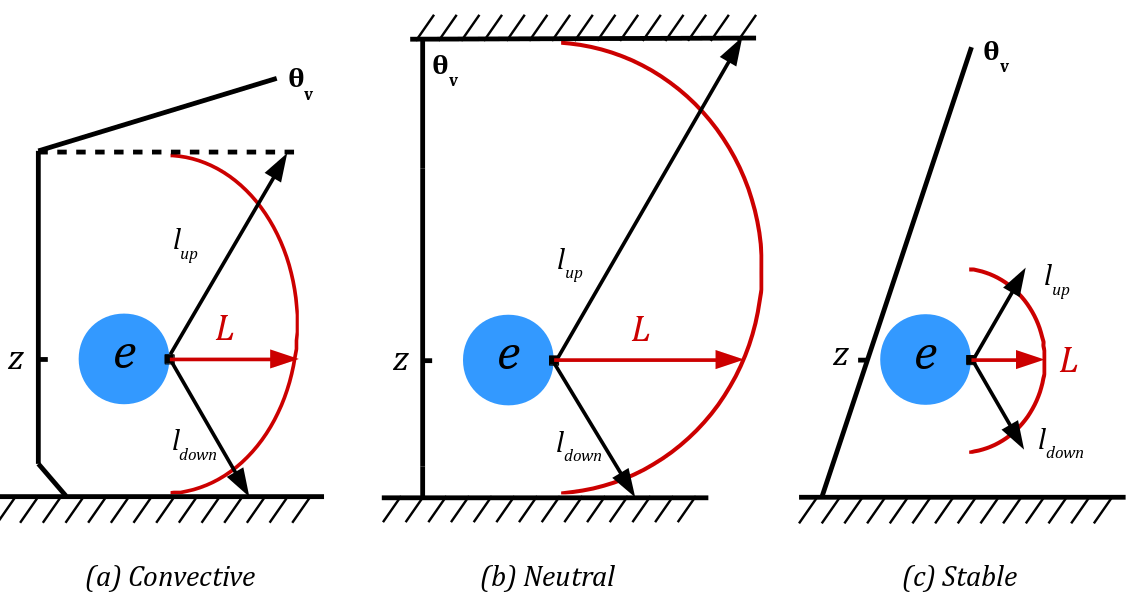
\includegraphics[width = 16cm]{\EPSDIR/BL89.png}
\caption{BL89 mixing length vertical profile (red) in convective, neutral and stable boundary layers.}
\label{fig:BL89}
\end{figure}

To improve the representation of turbulent mixing in neutral and stable boundary layers, RM17 (Rodier and Masson, 2017) adds a local vertical wind shear term to the buoyancy-based BL89 formulation :
\begin{equation}
\begin{split}
\int_z^{z+l_{up}} \left[\dfrac{g}{\theta_{vref}}(\theta_v (z) - \theta_v (z')) + C_0 \sqrt{e}S(z')\right]dz' = - e(z), \\
\int_{z-l_{down}}^z \left[\dfrac{g}{\theta_{vref}}(\theta_v (z') - \theta_v (z))+ C_0 \sqrt{e}S(z')\right]dz' = - e(z),
\end{split}
\label{eq:BS}
\end{equation}

where $C_0$ is a constant and $S(z')$ the local vertical wind shear:

\begin{equation}
S = \sqrt{\left(\dfrac{\partial \overline{u}}{\partial z}\right)^2 + \left(\dfrac{\partial \overline{v}}{\partial z}\right)^2}
\end{equation}

The shear term corresponds to the slowdown effect produced by the vertical decoupling of turbulent structures when the local shear is strong (Figure \ref{fig:shear}). This effect also depends on the average eddy size with larger eddies more decoupled.

\begin{figure}[!ht]
\centering
\noindent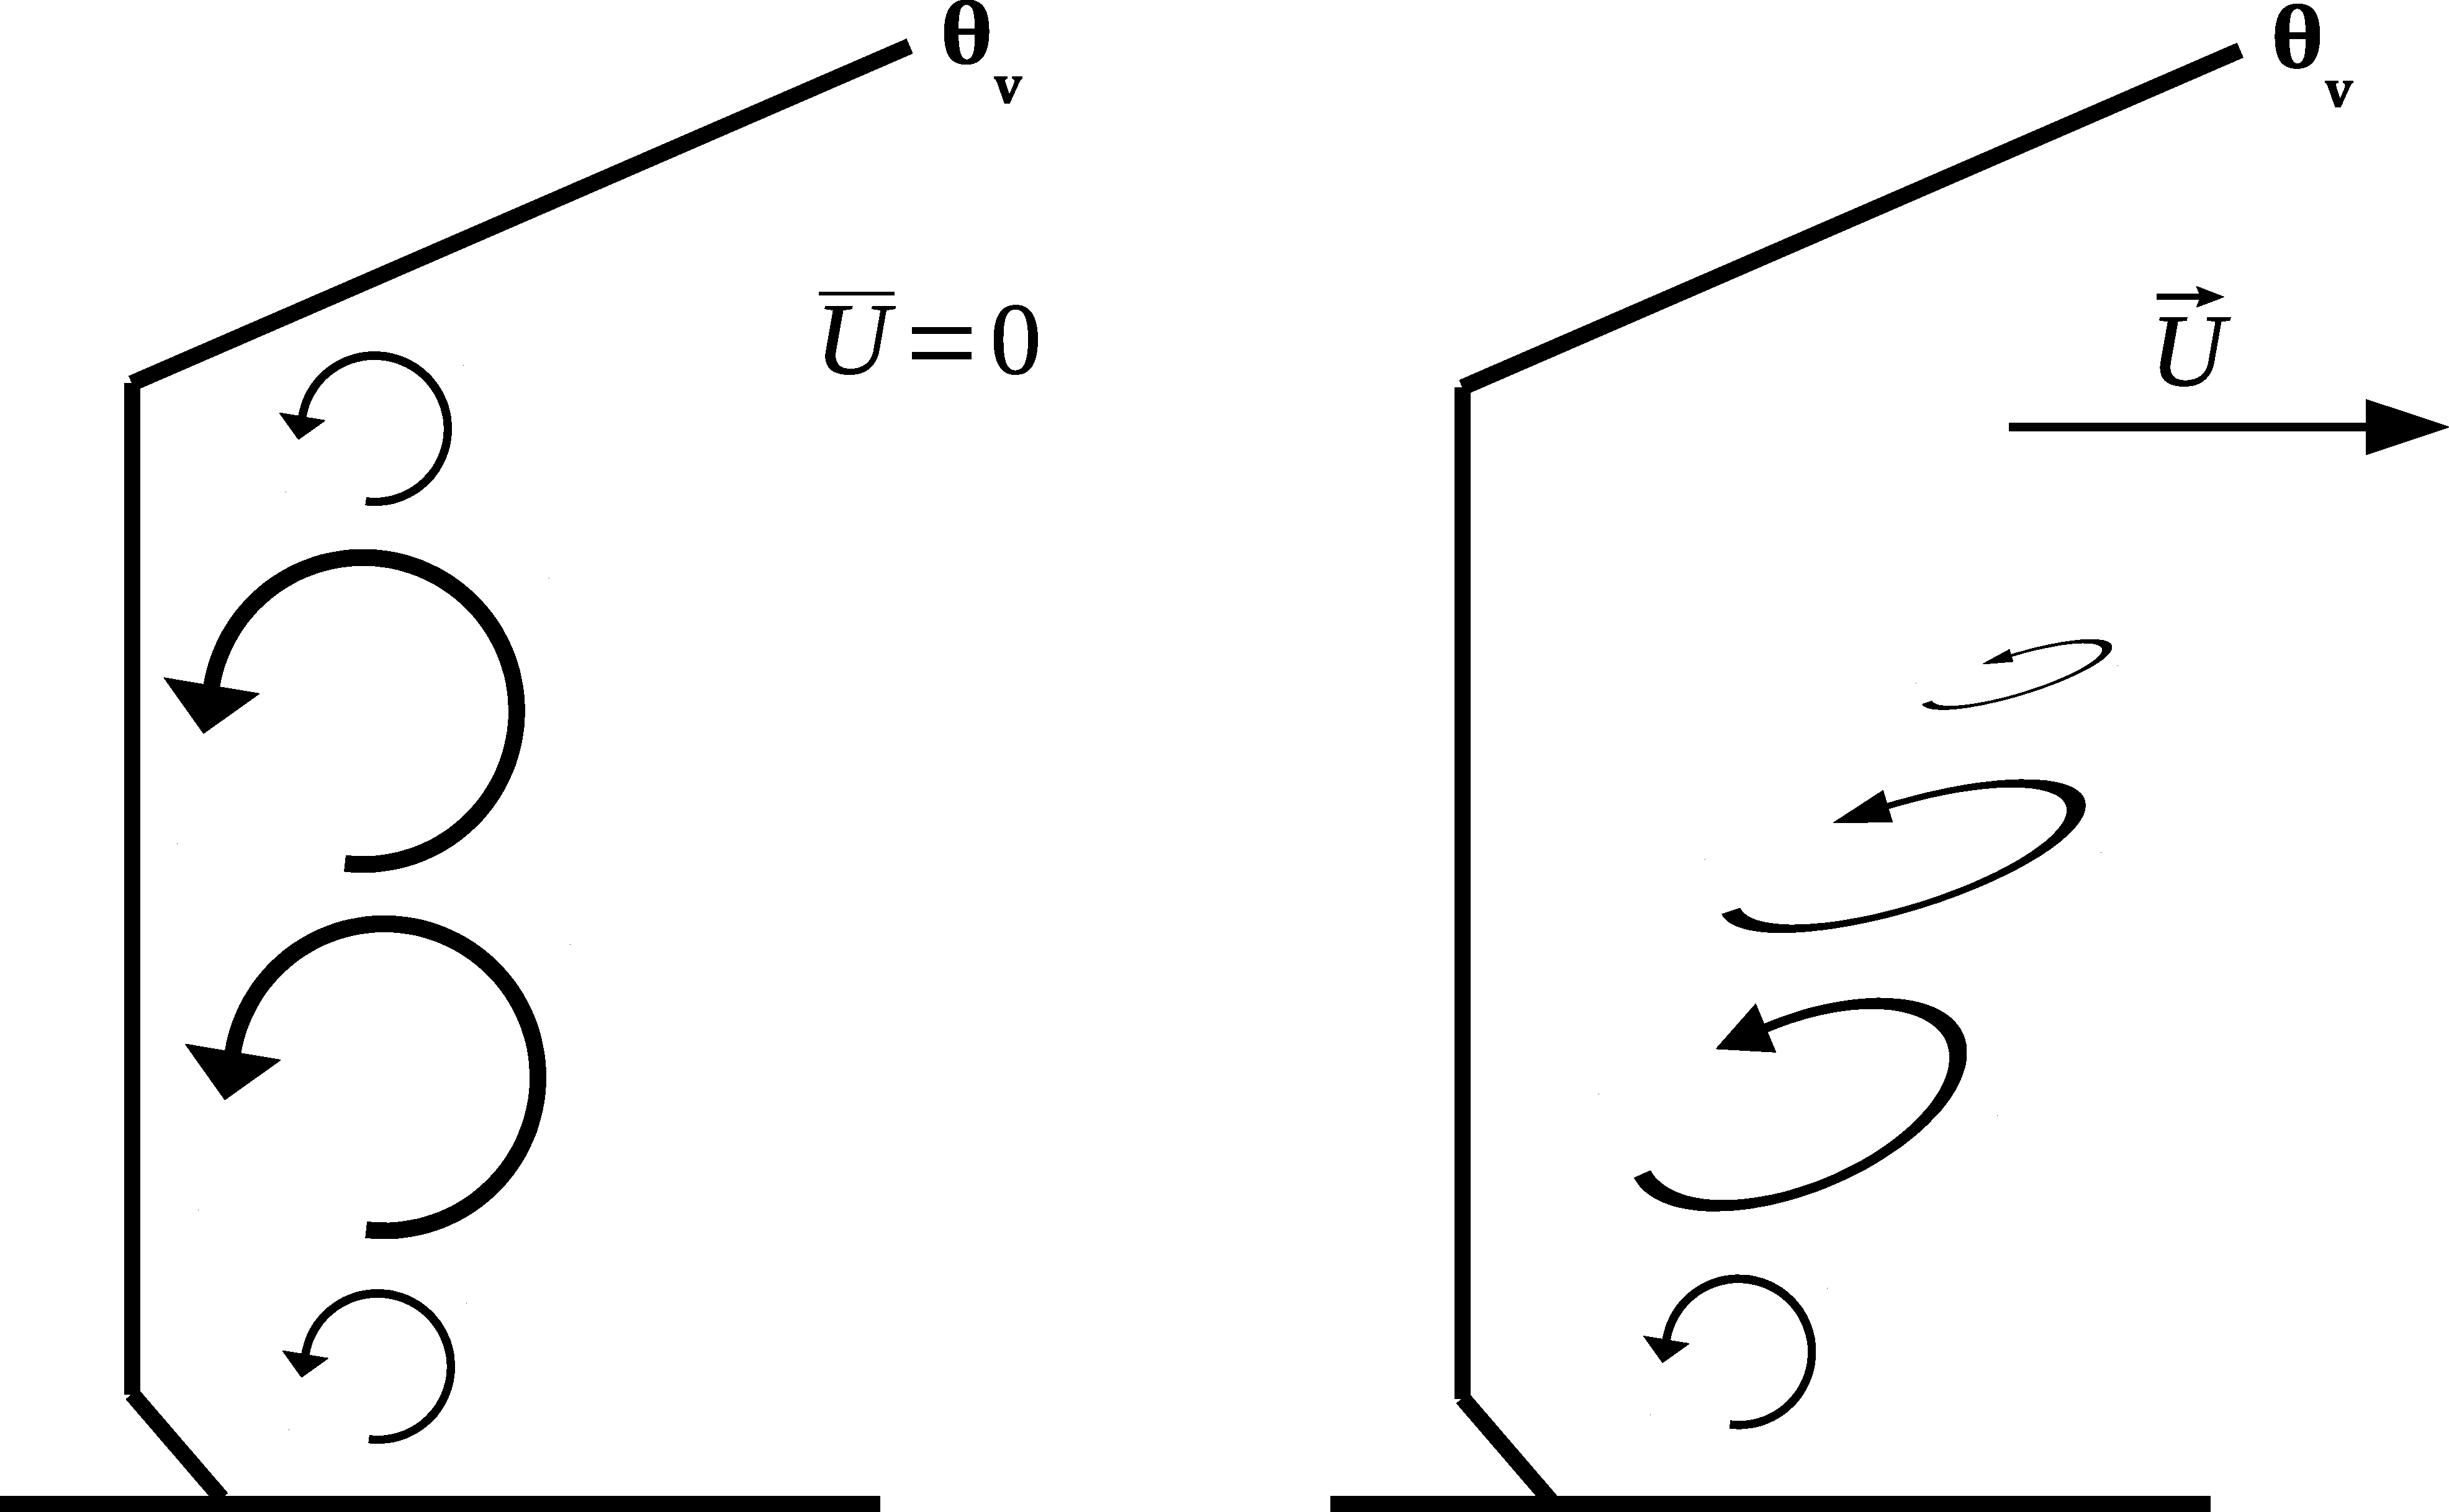
\includegraphics[width=8.5cm]{\EPSDIR/BS.jpg}
\caption{Schematic view of the effect of stratification and vertical wind shear on the reduction of the vertical mixing efficiency. Without wind shear (left), the turbulent structures are constrained by the distance to the surface and by the stratification. The presence of a wind shear (right) results in the stretching and vertical decoupling of the turbulent structures.}
\label{fig:shear}
\end{figure}

\subsection{Qualitative behavior of the 1D dry system with BL length}
\paragraph{Critical Richardson number}
Let us write the 1D TKE evolution equation introducing into it the expressions
for the fluxes, and neglecting the turbulent transport for this particular case:
%PM 02/07/2001 D�but diverses retouches Pascal Marquet
\be
\frac {\partial e}{\partial t}=
\frac{4 L}{15 C_m} e^{\frac{1}{2}} (\frac {\partial U}{\partial z})^2
-\frac{g}{\theta_{v0}}\frac{2 L}{3 C_s} e^{\frac{1}{2}}
 \frac {\partial \theta}{\partial z}
 \left(1+C_1  \frac{L^2}{e} \frac{g}{\theta_{v0}}
       \frac {\partial \theta}{\partial z}
 \right)^{-1}
- C_{\epsilon} \frac{e^{\frac{3}{2}}}{L}
\ee

\noindent
where the term $(\,\,\,\,)^{-1}$ is the developed expression for $\phi_3$ in
1D dry mode. Introducing the value for BL in stable layers
($ L= \sqrt{\frac{2 e(z)}{\alpha \beta}}$) and defining the buoyancy as
$B=\beta \alpha$,

\be
\frac {\partial e}{\partial t}= e \left[
\frac {4 \sqrt{2}}{15 C_m} (\frac {\partial U}{\partial z})^2 \frac{1}{\sqrt{B}}
-\sqrt{B}\sqrt{2} \frac{2}{3 C_s} (\frac{1}{1+2C_1})
- \frac{C_{\epsilon}}{\sqrt{2}} \sqrt{B} \right]
\ee
%PM 02/07/2001 Fin diverses retouches Pascal Marquet\noindent

The critical Richardson number is the one that nullifies the previous equation,
\be
Ri_c= \frac{B}{(\frac {\partial U}{\partial z})^2}=
\frac  {\frac {4 \sqrt{2}}{15 C_m} }
       { \frac{2 \sqrt{2}}{3 C_s} (\frac{1}{1+2C_1}) + \frac{C_{\epsilon}}{\sqrt{2}}}
\ee

\noindent
and entering the values of the constants (RS81), $C_m=C_s=4, C_1=0.139,
C_{\epsilon}=0.7$, the critical Richardson of the 1D proposed scheme is
{\bf $Ri_c= 0.139$}.

\subsection{Mixing length in clouds}
From the masdev46 version a namelist {\tt NAM\_TURB\_CLOUD} allows us to differentiate the mixing length inside and outside a cloud, for the chosen model {\tt NMODEL\_CLOUD}.
Indeed, in a convective atmosphere, the cloud interface (but also inside the cloud)  undergoes a small scale instabilities of a few meters which enhances the mixing (Squire 1958; Klaassen and Clark 1985; Emanuel 1994). The clear sky mixing length cannot be sufficient to take into account this turbulence enhancement when the physical gradients are not resolved.
The proposed simple solution consists in chosen a specific cloud mixing length ({\tt CTURBLEN\_CLOUD}) which can be increased in the 3D turbulence scheme following an instability criterion. At each time step and in each horizontal direction, if a grid point satisfies all the following conditions:
\begin{itemize}
\item itself or its adjacent points are cloudy ($r_c+r_i>0.001$~g/kg);
\item G, the horizontal gradient of the non precipitating total water
($r_v+ r_c+r_i$) is strong enough ($|G|\leq 0.1$~g/kg/km);
\item G amplifies itself with time by advection, that is to say the
frontogenetic type term $Q=dG/dt$ is of the same sign as $G$.
\end{itemize}
The mixing length at this point which appears in the diffusion coefficient $K=L\sqrt{e}$ of the horizontal fluxes is multiplied by the coefficient $\alpha$, a linear function of $Q$ (averaged in both horizontal directions) between two limits to be prescribed in the namelist ($Q_{\rm min}$  and $Q_{\rm max}$), with a maximum $\alpha_{\rm max}$ also to choose (Fig.~\ref{coef_ampl_incloud}).
This local enhancement of the mixing length in clouds has been tested at resolutions of 2-3~km in a thunderstorm with extreme vertical velocities. With the following values, taken by default in the namelist, the vertical velocities and fluxes are reasonable compared to the high resolution simulation (400~m): $\alpha_{\rm max}=5$, $Q_{\rm min}=0.001$~g/kg/km/s,  $Q_{\rm max}=0.01$~g/kg/km/s.

\begin{figure}[!ht]
\centerline{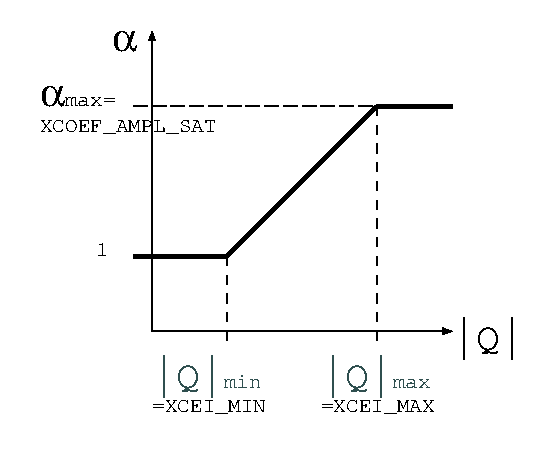
\includegraphics[width=10cm]{\EPSDIR/coef_ampl_incloud.eps}}
\caption{Coefficient $\alpha$ of in-cloud mixing length enhancement as function of the instability criterion $Q$.}
\label{coef_ampl_incloud}
\end{figure}

\section{Closure by dissipation equation}

This is an alternative way to close the system (Hanjalic and Launder 1972),
obtaining a value for L from an additional prognostic equation. The most
popular method is the so-called $k-\epsilon$ approach, in the
engineering vocabulary, where $k$ stands for the TKE and $\epsilon$ for
its dissipation.

The prognostic equation for $\epsilon$ reads
\begin{equation}
\frac {D \epsilon}{D t}=P(\epsilon)-D(\epsilon) + T(\epsilon),
\end{equation}
where the source terms are defined as
\begin{eqnarray}
P(\epsilon)&=&-C_{\epsilon 1} \frac {\epsilon}{e} \overline{u_i' u_k'}
\frac{\partial U_i}{\partial x_k}=C_{\epsilon 1} \frac {\epsilon}{e}
P(e),\\
D(\epsilon)&=&C_{\epsilon 2} \frac {\epsilon ^2}{e},\\
T(\epsilon)&=&-\frac{\partial}{\partial x_j}
(-c_{\epsilon} \frac{e}{\epsilon} \overline{u_j' u_k'}
\frac{\partial \epsilon}{\partial x_k})=-\frac{\partial
\overline{w' \epsilon'}}{\partial z}
\end{eqnarray}

However, in the presence of stratification Duynkerke (1988) showed that
it is necessary to use
\begin{equation}
P(\epsilon)=S+\max(0,B)+\max(0,T(e))
\end{equation}
where S, B and T stand for the shear production, buoyancy production and
turbulent transport in the TKE evolution equation.\\
\nocite{Han_Laun72} \nocite{Duynkerke88}

Knowing $\epsilon$, the mixing length is recovered by inverting the
Kolmogorov relation
\begin{equation}
\epsilon=C_{\epsilon} \frac{e^{\frac{3}{2}}}{L}.
\end{equation}

Although it has been coded, this formulation is not yet giving satisfactory
results, and is not currently available.


%\chapter{Inclusion of a dissipative heating term in M\'esoNH}

%{\em by J.-P. Pinty}

\section{Conservation of the energy in Meso-NH}

The examination of the energy conservation in a model of atmosphere is a very
difficult task. In numerical models, this question is even untractable. However,
a recent study of Blister and Emanuel (1998) pointed out that a thermodynamic
energy arising from dissipative heating is always neglected in mesoscale
models. Indeed this should not be the case when simulating hurricanes or very turbulent 
flows as omitting this term may lead to an appreciable underestimation of the intensity of 
tropical cyclones.

It is well known that the frictional dissipation of kinetic energy occurs at 
molecular scales where it is ultimately converted into thermal energy or heat.
As numerical models perform a time integration of the "mean" (grid-averaged)
momentum equations, an additional equation is used to parameterize the sub-grid 
scale motions and their up-scaling fluxes. 

The momentum conservation equation is rewritten here for convenience:
\begin{eqnarray}
\label{NewEqMomentum}
\dfrac{\partial}{\partial t}(\rho_{d\,eff} {U_i})
+\dfrac{\partial}{\partial x_j} (\rho_{d\,eff} {U_i} \cdot {U_j} )
%+\rho_{d\,eff} C_{pd} \theta_{v}\overbar{ \nabla} \Pi '
+ \rho_{d\,eff} {\cal F}_{\Pi}
+ \rho_{d\,eff}  \delta_{i3} g \dfrac{\theta_v-\theta_{v\,ref}}{\theta_{v\,ref}}
+ \rho_{d\,eff} f \epsilon_{ij3} {U_j} = & \nonumber\\
+ \nu \dfrac{\partial^2}{\partial x_j^2} (\rho_{d\,eff} {U_i}) 
+ \rho_{d\,eff} {\cal F} , \qquad &
\end{eqnarray}

\noindent where $\rho_{d\,eff} \vec{{\cal F}_{\Pi}}$ is the pressure gradient force, which
takes different forms in the three anelastic systems:

%
\parbox{12cm}{
\begin{displaymath}
\rho_{d\,eff} \vec{{\cal F}_{\Pi}} =  \left\{
\begin{array}{l@{\quad}cc}
\rho_{d\,eff}  \vec{ \nabla}(C_{pd} \theta_{v\,ref} \Pi '),
                                        & \quad &\mbox{(Lipps-Hemler)}\\
\rho_{d\,eff} C_{pd} \theta_{v\,ref} \vec{ \nabla} \Pi ',
                                                & \quad &\mbox{(Mod. Anelastic  Eq.)} \\
\rho_{d\,eff} C_{pd} \theta_{v} \vec{ \nabla} \Pi '. & \quad  &\mbox{(Durran)}
\end{array}
\right.
\end{displaymath}
}
\hfill
\parbox{1cm}{
\begin{eqnarray}
\ \label{LhgradP} \\ \label{MAEgradP}   \\ \label{DUgradP}
\end{eqnarray}
}
%

Expansion of the mean and turbulent parts ($U_i=\overline{U_i}+u'_i$) and
applying Reynolds averaging rules on the momentum equation leads to
\begin{eqnarray}
\label{NewMeanEqMomentum}
\dfrac{\partial}{\partial t}(\rho_{d\,eff} \overline{U_i})
+\dfrac{\partial}{\partial x_j} (\rho_{d\,eff} \overline{U_i} \cdot \overline{U_j} )
+ \rho_{d\,eff} \overline{\cal F}_{\Pi}
+ \rho_{d\,eff}  \delta_{i3} g \dfrac{\overline{\theta_v}-\theta_{v\,ref}}{\theta_{v\,ref}}
+ \rho_{d\,eff} f \epsilon_{ij3} \overline{U_j} = & \nonumber\\
+ \nu \dfrac{\partial^2}{\partial x_j^2} (\rho_{d\,eff} \overline{U_i}) -\dfrac{\partial}{\partial x_j} (\rho_{d\,eff} \overline{u'_i u'_j})               
+ \rho_{d\,eff} \overline{\cal F} , \qquad &
\end{eqnarray}

\noindent where $\rho_{d\,eff} \overline{u'_i u'_j}$ is the turbulent mean 
flux. The conservation equation of the turbulent part is obtained by 
subtracting equation (\ref{NewMeanEqMomentum}) to (\ref{NewEqMomentum})
\begin{eqnarray}
\label{NewTurbEqMomentum}
\dfrac{\partial}{\partial t}(\rho_{d\,eff} {u'_i})
+\dfrac{\partial}{\partial x_j} (\rho_{d\,eff} {u'_i} \cdot \overline{U_j} )
+ \rho_{d\,eff} ({\cal F}_{\Pi})'
+ \rho_{d\,eff}  \delta_{i3} g \dfrac{\theta'_v}{\theta_{v\,ref}}
+ \rho_{d\,eff} f \epsilon_{ij3} {u'_j} = 
 & \nonumber\\
- \dfrac{\partial}{\partial x_j} (\rho_{d\,eff} u'_i u'_j) 
- \dfrac{\partial}{\partial x_j} (\rho_{d\,eff} \overline{U_i} \cdot {u'_j} )
\qquad  & \nonumber\\
+ \nu \dfrac{\partial^2}{\partial x_j^2} (\rho_{d\,eff} {u'_i}) 
+ \dfrac{\partial}{\partial x_j} (\rho_{d\,eff} \overline{u'_i u'_j}) 
+ \rho_{d\,eff} ({\cal F})' , \qquad &
\end{eqnarray}

Multiplying equation (\ref{NewMeanEqMomentum}) by $\overline{U_i}$ leads to the
mean kinetic energy equation with 
$K=\rho_{d\,eff} (\overline{U_i} \cdot \overline{U_i}/2)$
and using the anelastic continuity equation 
$\partial/\partial x_i (\rho_{d\,eff} \overline{U_i})=0$ of the mean flow
\begin{eqnarray}
\label{NewMeanEqKenergy}
\dfrac{\partial}{\partial t} K
+\dfrac{\partial}{\partial x_j} (K \cdot \overline{U_j} )
+ \Big[\rho_{d\,eff} \overline{\cal F}_{\Pi}
+ \rho_{d\,eff}  \delta_{i3} g \dfrac{\overline{\theta_v}-\theta_{v\,ref}}{\theta_{v\,ref}}
+ \rho_{d\,eff} f \epsilon_{ij3} \overline{U_j} \Big] \cdot \overline{U_i} = & \nonumber\\
+\Big[\nu \dfrac{\partial^2}{\partial x_j^2} (\rho_{d\,eff} \overline{U_i}) -\dfrac{\partial}{\partial x_j} (\rho_{d\,eff} \overline{u'_i u'_j})               
+ \rho_{d\,eff} \overline{\cal F} \Big] \cdot \overline{U_i} , \qquad &
\end{eqnarray}
\noindent while multiplying equation (\ref{NewTurbEqMomentum}) by $u'_i$ and 
averaging after rearrangement leads to the turbulent kinetic energy equation 
with $TKE=\rho_{d\,eff} (\overline{u'_iu'_i}/2)$ (the anelastic continuity 
equation 
$\partial/\partial x_i (\rho_{d\,eff} {u'_i})=0$ of the turbulent flow is 
used)
\begin{eqnarray}
\label{NewTurbEqTKE}
\dfrac{\partial}{\partial t} TKE
+\dfrac{\partial}{\partial x_j} (TKE \cdot \overline{U_j} )
+ \rho_{d\,eff} \overline{({\cal F}_{\Pi})'u'_i}
+ \rho_{d\,eff}  \delta_{i3} g \dfrac{\overline{\theta'_v u'_i}}{\theta_{v\,ref}}
+ \rho_{d\,eff} f \epsilon_{ij3} \overline{u'_i u'_j} = & \nonumber\\
- \overline{u'_i\dfrac{\partial}{\partial x_j} (\rho_{d\,eff} u'_i u'_j)} 
- \overline{u'_i \dfrac{\partial}{\partial x_j} (\rho_{d\,eff} \overline{U_i} \cdot {u'_j} )}
+ \nu \overline{u'_i \dfrac{\partial^2}{\partial x_j^2} (\rho_{d\,eff} {u'_i})} 
+ \rho_{d\,eff} \overline{({\cal F})' u'_i} , \qquad &
\end{eqnarray}
\noindent which is equivalent to:
\begin{eqnarray}
\label{NewNewTurbEqTKE}
\dfrac{\partial}{\partial t} TKE
+\dfrac{\partial}{\partial x_j} (TKE \cdot \overline{U_j} )
+ \rho_{d\,eff} \overline{({\cal F}_{\Pi})'u'_i}
+ \rho_{d\,eff}  \delta_{i3} g \dfrac{\overline{\theta'_v u'_i}}{\theta_{v\,ref}}
+ \rho_{d\,eff} f \epsilon_{ij3} \overline{u'_i u'_j} = & \nonumber\\
- \dfrac{\partial}{\partial x_j} \overline{TKE' u'_j}
- (\rho_{d\,eff} \overline{u'_i u'_j}) \dfrac{\partial}{\partial x_j} \overline{U_i} 
\qquad  & \nonumber\\
+ \dfrac{\nu}{\rho_{d\,eff}} \Big[ \dfrac{\partial}{\partial x_j} \rho_{d\,eff} \Big[ \dfrac{\partial}{\partial x_j} TKE\Big] \Big]
- \dfrac{\nu}{\rho_{d\,eff}} \Big[ \overline{\dfrac{\partial}{\partial x_j} \Big( \rho_{d\,eff} u'_i\Big)} \Big]^2
+ \rho_{d\,eff} \overline{({\cal F})' u'_i} , \qquad &
\end{eqnarray}
\noindent where the flux-like notation $\overline{TKE' u'_j}$ stands for 
$\rho_{d\,eff} \overline{(u'_iu'_i/2) u'_j}$. In the rhs of equation 
(\ref{NewNewTurbEqTKE}), the $TKE$-diffusion term, proportional to the molecular
viscosity $\nu$, is split in two terms. The "Laplacian" term is a redistribution
term which is often neglected. The second term is much larger and is always 
negative (minus a squared quantity). This term corresponds to the viscous 
dissipation rate $\varepsilon$ 
\begin{equation}
\label{DissipationTerm}
\varepsilon_{TKE} = \dfrac{\nu}{\rho_{d\,eff}} \Big[ \overline{\dfrac{\partial}{\partial x_j} \Big( \rho_{d\,eff} u'_i\Big)} \Big]^2,
\end{equation}
Adding equations (\ref{NewMeanEqKenergy}) and (\ref{NewNewTurbEqTKE}) gives the
evolution of the total kinetic energy equation ($K + TKE$) which explicitly 
contains the momentum
dissipation term $\varepsilon$. By virtue of the total energy conservation, a
counterpart dissipative energy must be added to the thermodynamic equation. 
This can be simply done by the introduction of a dissipative heating term of
the form
\begin{eqnarray}
\label{NewThequa}
\dfrac{\partial}{\partial t}(\rho_{d\,eff} \theta)  + \vec{ \nabla} \cdot
(\rho_{d\,eff} \theta \;\vec{U})
= 
%% \rho_{d\,eff} \left[ {R_d+r_vR_v\over R_d}{C_{pd} \over C_{ph}}-1 \right]
%% {\theta \over \Pi_{ref}} w {\partial \Pi_{ref} \over \partial z}
%% \nonumber \\
%% + {\rho_{d\,eff}\over \Pi_{ref} C_{ph}} \left[
%%  L_m {D(r_i+r_s+r_g+r_h)\over Dt} - L_v {Dr_v\over Dt} + {\cal H}  \right].
\cdots + \dfrac{\rho_{d\,eff} \varepsilon_{e}}{\Pi_{ref} C_{ph}}.
\end{eqnarray}
The turbulence scheme in Meso-NH is based on a turbulent kinetic
equation of $e$ defined as $e=TKE/\rho_{d\,eff}$. Most of the second order 
terms in equation (\ref{NewNewTurbEqTKE}) including 
$\varepsilon_{TKE}= \varepsilon_{e}\times \rho_{d\,eff}$ are parameterized 
according to Cuxart et al. (2000).

\section{Terrain-following coordinate system}

In Meso-NH, the coordinate system is not Cartesian, in order to account
for steep terrain, and the sphericity of the earth. As explained in Part I,
Chapters 3 and 4 on coordinate systems and discretization, respectively,
we use a $(\overline{x},\overline{y},\overline{z})$ coordinate
system, and the contravariant components of the velocity. By inserting these
various elements in the basic equations, the form of the turbulent terms
is readily obtained. For instance, the turbulent terms in the equation
for the mean $x$ momentum component read
\begin{eqnarray}
{\partial \tilde{\rho} \overline{u}\over \partial t}=\cdots
&-&\left[\frac{\partial}{\partial \overline{x}}(\tilde{\rho}
\frac{\overline{u'u'}}{d_{xx}})+\frac{\partial}{\partial \overline{y}}
(\tilde{\rho}\frac{\overline{u'v'}}{d_{yy}})+
\frac{\partial}{\partial \overline{z}}(\tilde{\rho}\frac{\overline{w'u'}}
{d_{zz}}-\tilde{\rho}\overline{u'u'}\frac{d_{zx}}{d_{xx}d_{zz}}
-\tilde{\rho}\overline{v'u'}\frac{d_{zy}}{d_{yy}d_{zz}}) \right ]\nonumber\\
&+&\overline{u'v'}\frac{\tilde{\rho}cos\gamma}{rcos\varphi}(sin \varphi -K)
+\overline{v'v'}\frac{\tilde{\rho}sin\gamma}{rcos\varphi}(sin \varphi -K)
-\tilde{\rho}\frac{\overline{u'w'}}{r}.
\end{eqnarray}
The last line of this expression  arises from the curvature terms
generated by the sphericity of the Earth.
In the following, we will assume that these sphericity terms have negligible
contributions on the turbulence, and therefore ignore them.

On the other hand, we should stress that the $(u,v,w)$ used in the equations
are still the Cartesian components of the velocity.
So, the terms that the turbulence scheme will supply to Meso-NH are
\begin{eqnarray}
\frac{\partial }{\partial t}(\tilde{\rho}u)&=
\cdots&-\left[\frac{\partial}{\partial \overline{x}}(\tilde{\rho}
\frac{\overline{u'u'}}{d_{xx}})+\frac{\partial}{\partial \overline{y}}(\tilde
{\rho}\frac{\overline{u'v'}}{d_{yy}})+
\frac{\partial}{\partial \overline{z}}(\tilde{\rho}\frac{\overline{w'u'}}
{d_{zz}}-\tilde{\rho}\overline{u'u'}\frac{d_{zx}}{d_{xx}d_{zz}}
-\tilde{\rho}\overline{v'u'}\frac{d_{zy}}{d_{yy}d_{zz}}) \right ],\nonumber\\
\frac{\partial }{\partial t}(\tilde{\rho}v)&=
\cdots&-\left[\frac{\partial}{\partial \overline{x}}(\tilde{\rho}
\frac{\overline{u'v'}}{d_{xx}})+\frac{\partial}{\partial \overline{y}}(\tilde
{\rho}\frac{\overline{v'v'}}{d_{yy}})+
\frac{\partial}{\partial \overline{z}}(\tilde{\rho}\frac{\overline{v'w'}}
{d_{zz}}-\tilde{\rho}\overline{u'v'}\frac{d_{zx}}{d_{xx}d_{zz}}
-\tilde{\rho}\overline{v'v'}\frac{d_{zy}}{d_{yy}d_{zz}}) \right ],\nonumber\\
\frac{\partial }{\partial t}(\tilde{\rho}w)&=
\cdots&-\left[\frac{\partial}{\partial \overline{x}}(\tilde{\rho}
\frac{\overline{w'u'}}{d_{xx}})+\frac{\partial}{\partial \overline{y}}(\tilde
{\rho}\frac{\overline{w'v'}}{d_{yy}})+
\frac{\partial}{\partial \overline{z}}(\tilde{\rho}\frac{\overline{w'w'}}
{d_{zz}}-\tilde{\rho}\overline{u'w'}\frac{d_{zx}}{d_{xx}d_{zz}}
-\tilde{\rho}\overline{v'w'}\frac{d_{zy}}{d_{yy}d_{zz}}) \right ],\nonumber \\
\frac{\partial }{\partial t}(\tilde{\rho}s)&=
\cdots&-\left[\frac{\partial}{\partial \overline{x}}(\tilde{\rho}
\frac{\overline{s'u'}}{d_{xx}})+\frac{\partial}{\partial \overline{y}}(\tilde
{\rho}\frac{\overline{s'v'}}{d_{yy}})+
\frac{\partial}{\partial \overline{z}}(\tilde{\rho}\frac{\overline{w's'}}
{d_{zz}}-\tilde{\rho}\overline{u's'}\frac{d_{zx}}{d_{xx}d_{zz}}
-\tilde{\rho}\overline{v's'}\frac{d_{zy}}{d_{yy}d_{zz}}) \right ],\nonumber
\end{eqnarray}
where $s$ is any scalar.

In addition, all the gradients appearing in the flux formulation and in the
TKE prognostic equation must be evaluated in the model coordinate system by
the chain rule (see below).

%%%%%%%%%%%%%%%%%%%%%%%%%%%%%%%%%%%%%%%%%%%%%%%%%%%%%%%%%%%%%%%%%%%%%%%%%%%%%

\section{Spatial discretization}
The location of the different variables on the computation grid is shown in
Fig.~\ref{maille}. All the variables shown share the same index values i,j,k.
In the following, we will use the Schuman discretization operators, as defined
in Part I, Chapter 4 on discretization (section 4.3).

\begin{figure}[!ht]
\centerline{\includegraphics[]{\EPSDIR/maille.eps}}
\caption{Location of variables on the grid for turbulence computation.}
\label{maille}
\end{figure}

The discretized form of the turbulence terms in the main equations reads
\begin{eqnarray}
\delta_t \left [ \overline{(\overline{\tilde{\rho}}^x u)}^t \right ]=
\cdots&-&\delta_x(\tilde{\rho}\frac{\overline{u'u'}}{\overline{d_{xx}}^x})
-\delta_y(\overline{\tilde{\rho}}^{x,y}\frac{\overline{u'v'}}{\overline{d_{yy}
}^x}) \nonumber \\
&-&\delta_z(\overline{\tilde{\rho}}^{z,x}\frac{\overline{w'u'}}{\overline
{d_{zz}}^x}
-\overline{\tilde{\rho}}^{z,x}\overline{\overline{u'u'}}^{z,x}
\frac{d_{zx}}{\overline{d_{xx}}^z\overline{d_{zz}}^x}
-\overline{\tilde{\rho}}^{z,x}\overline{\overline{v'u'}}^{z,y}
\frac{\overline{d_{zy}}^{x,y}}{\overline{d_{yy}}^{x,y,z}\overline{d_{zz}}^x}
) \nonumber\\
\delta_t \left [ \overline{(\overline{\tilde{\rho}}^y v)}^t \right ]=
\cdots&-&\delta_x(\overline{\tilde{\rho}}^{x,y}\frac{\overline{u'v'}}
{\overline{d_{xx}}^y})
-\delta_y(\tilde{\rho}\frac{\overline{v'v'}}{\overline{d_{yy}}^y})
\nonumber \\
&-&\delta_z(\overline{\tilde{\rho}}^{z,y}\frac{\overline{w'v'}}{\overline
{d_{zz}}^y}
-\overline{\tilde{\rho}}^{z,y}\overline{\overline{u'v'}}^{z,x}
\frac{\overline{d_{zx}}^{y,x}}{\overline{d_{xx}}^{xyz}\overline{d_{zz}}^y}
-\overline{\tilde{\rho}}^{z,y}\overline{\overline{v'v'}}^{z,y}
\frac{d_{zy}}{\overline{d_{yy}}^z\overline{d_{zz}}^y}
) \nonumber\\
\delta_t \left [ \overline{(\overline{\tilde{\rho}}^z w)}^t \right ]=
\cdots&-&\delta_x(\overline{\tilde{\rho}}^{z,x}\frac{\overline{u'w'}}
{\overline{d_{xx}}^z})
-\delta_y(\overline{\tilde{\rho}}^{z,y}\frac{\overline{v'w'}}{\overline{d_{yy}
}^z})
\nonumber \\
&-&\delta_z(\tilde{\rho}\frac{\overline{w'w'}}{\overline{d_{zz}}^z}
-\tilde{\rho}\overline{\overline{u'w'}}^{z,x}
\frac{\overline{{d_{zx}}^{x,z}}}{\overline{d_{xx}}^x\overline{d_{zz}}^z}
-\tilde{\rho}\overline{\overline{v'w'}}^{y,z}
\frac{\overline{d_{zy}}^{y,z}}{\overline{d_{yy}}^{x}\overline{d_{zz}}^z}
) \nonumber\\
\delta_t \left [ \overline{(\tilde{\rho} s)}^t \right ]=
\cdots&-&\delta_x(\overline{\tilde{\rho}}^x\frac{\overline{u's'}}{d_{xx}})
-\delta_y(\overline{\tilde{\rho}}^y\frac{\overline{v's'}}{d_{yy}})
\nonumber \\
&-&\delta_z(\overline{\tilde{\rho}}^z\frac{\overline{w's'}}{d_{zz}}
-\overline{\tilde{\rho}}^z\overline{\overline{u's'}}^{z,x}
\frac{\overline{d_{zx}^x}}{\overline{d_{xx}}^{z,x}d_{zz}}
-\overline{\tilde{\rho}}^z\overline{\overline{v's'}}^{z,y}
\frac{\overline{d_{zy}}^y}{\overline{d_{yy}}^{z,y}d_{zz}}  )
\label{discturb}
\end{eqnarray}
\\

Here, we have assumed that the time discretization is fully explicit, and all
the terms on the right hand side are taken at time $t-\Delta t$. As
explained in the final section however, we allow for some degree of implicitness
in the time discretization of the purely vertical diffusion terms, in order
to allow for longer time steps when the model is used in meso-scale mode.
\\

In (\ref{discturb}), we still use the expression of the
turbulent fluxes in the Cartesian frame. Those must be expressed as a function
of the gradients of the mean variables in the Cartesian frame. To ease this
formulation, we have developed 15 different "Cartesian gradient operators",
depending of the direction in which the gradient is taken, and the precise
locations on the grid where the  information is available. The generic notation
for these operators is $GX_i\_A\_B$: $X_i$ refers to the (Cartesian) direction
where the gradient is taken, $A$ to the variable location, and $B$ to the
location where the gradients must be known. The detailed expression of these
operators is the following.
\\
\\
\noindent
1) Gradients at mass points for variables located at mass points:
\begin{eqnarray}
\frac{\partial \bullet}{\partial x}&=
\frac{1}{\overline{d_{xx}}^x}\left[ \delta_x \overline{\bullet}^x -
\overline{\left({\overline{d_{zx}}^x \delta_z \bullet \over d_{zz}}\right) }^z
\right]
&\equiv GX\_M\_M
\nonumber\\
\frac{\partial \bullet}{\partial y}&=
\frac{1}{\overline{d_{yy}}^y}\left[ \delta_y \overline{\bullet}^y -
\overline{\left({\overline{d_{zy}}^y \delta_z \bullet \over d_{zz}}\right) }^z
\right]
&\equiv GY\_M\_M
\nonumber\\
\frac{\partial \bullet}{\partial z}&=
\overline{\left( {\delta_z \bullet \over d_{zz} } \right) }^z
&\equiv GZ\_M\_M
\end{eqnarray}

\noindent
2) Gradients at wind points for variables located at mass points:
($\overline{u_i'\theta'}\Longleftrightarrow \frac{\partial \theta}{\partial x_i}$)
\begin{eqnarray}
\frac{\partial \bullet}{\partial x}&=
\frac{1}{d_{xx}}\left[ \delta_x \bullet -
\overline{\left({ d_{zx}\overline{\delta_z \bullet}^x \over d_{zz}}\right)}^z
\right]
&\equiv GX\_M\_U
\nonumber\\
\frac{\partial \bullet}{\partial y}&=
\frac{1}{d_{yy}}\left[ \delta_y \bullet -
\overline{\left({ d_{zy}\overline{\delta_z \bullet}^y \over d_{zz}}\right)}^z
\right]
&\equiv GY\_M\_V
\nonumber\\
\frac{\partial \bullet}{\partial z}&=
\frac{1}{d_{zz}} \delta_z \bullet
&\equiv GZ\_M\_W
\end{eqnarray}

\noindent
3) Gradients at mass points of variables located at wind points:
($\overline{u_i'^2} \Longleftrightarrow \frac{\partial u_i}{\partial x_i}$
unsummed)
\begin{eqnarray}
\frac{\partial \bullet}{\partial x}&=
\frac{1}{\overline{d_{xx}}^x}\left[ \delta_x \bullet -
\overline{\left({\overline{d_{zx}\delta_z \bullet}^x \over d_{zz}}\right)}^z
\right]
&\equiv GX\_U\_M
\nonumber\\
\frac{\partial \bullet}{\partial y}&=
\frac{1}{\overline{d_{yy}}^y}\left[ \delta_y \bullet -
\overline{\left({\overline{d_{zy}\delta_z \bullet}^y \over d_{zz}}\right)}^z
\right]
&\equiv GY\_V\_M
\nonumber\\
\frac{\partial \bullet}{\partial z}&=
\frac{1}{\overline{d_{zz}}^z} \delta_z \bullet
&\equiv GZ\_W\_M
\end{eqnarray}

\noindent
4) Gradients at vorticity points for variables located at wind points:
($\overline{u_i'u_j'} \Longleftrightarrow
\frac{\partial u_i}{\partial x_j}\,,\frac{\partial u_j}{\partial x_i}$)\\
For gradients localized at point UV:
\begin{eqnarray}
\frac{\partial \bullet}{\partial x}&=
\frac{1}{\overline{d_{xx}}^y}\left[ \delta_x \bullet -
\overline{\overline{\left({\delta_z\bullet \over \overline{d_{zz}}^y}\right)}^x
\overline{d_{zx}}^y }^z \right]
&\equiv GX\_V\_UV
\nonumber\\
\frac{\partial \bullet}{\partial y}&=
\frac{1}{\overline{d_{yy}}^x}\left[ \delta_y \bullet -
\overline{\overline{\left({\delta_z\bullet \over \overline{d_{zz}}^x}\right)}^y
\overline{d_{zy}}^x }^z \right]
&\equiv GY\_U\_UV
\end{eqnarray}

\noindent
For gradients localized at point UW:
\begin{eqnarray}
\frac{\partial \bullet}{\partial x}&=
\frac{1}{\overline{d_{xx}}^z}\left[ \delta_x \bullet -
\overline{\left({\overline{\delta_z\bullet}^z \over d_{zz}}\right)}^x d_{zx}
\right]
&\equiv GX\_W\_UW
\nonumber\\
\frac{\partial \bullet}{\partial z}&=
\frac{\delta_z\bullet}{\overline{d_{zz}}^x}
&\equiv GZ\_U\_UW
\end{eqnarray}

\noindent
For gradients localized at point VW:
\begin{eqnarray}
\frac{\partial \bullet}{\partial y}&=
\frac{1}{\overline{d_{yy}}^z}\left[ \delta_y \bullet -
\overline{\left({\overline{\delta_z\bullet}^z \over d_{zz}}\right)}^y d_{zy}
\right]
&\equiv GY\_W\_VW
\nonumber\\
\frac{\partial \bullet}{\partial z}&=
\frac{\delta_z\bullet}{\overline{d_{zz}}^y}
&\equiv GZ\_V\_VW
\end{eqnarray}

\smallskip
Making use of these operators, the discretized form of the turbulent
fluxes in the Cartesian frame reads as follows:
\begin{eqnarray}
\overline{u_i'\,u_j'}&=&\frac{2}{3}\delta_{ij}\,\overline{e}^{x_i,x_j}
 -\frac{4}{15} \frac{\overline{L}^{x_i,x_j}}{C_m} \overline{e^
{\frac{1}{2}}}^{x_i,x_j}
[ GX_j\_U_i\_U_iU_j(u_i)+GX_i\_U_j\_U_iU_j(u_j)\nonumber \\
&-&\frac{2}{3}\delta_{ij}\sum_{m=1}^{3} GX_m\_U_m\_U_iU_j(u_m) ] \\
\overline{u_i'\theta'}&=&-\frac{2}{3}\frac{\overline{L}^{x_i}}{C_s}
\overline{e^{\frac{1}{2}}}^{x_i}
GX_i\_M\_U\_i(\theta) \phi_i\\
\overline{u_i'r_v'}&=&-\frac{2}{3}\frac{\overline{L}^{x_i}}{C_s}
\overline{e^{\frac{1}{2}}}^{x_i}
GX_i\_M\_U\_i(r_v) \psi_i\\
\overline{\theta'r_v'}&=&C_2 L^2
\sum_{m=1}^{3}GX_m\_M\_M(\theta)GX_m\_M\_M(r_v)(\overline{\phi_m}^z
+\overline{\psi_m}^z)\\
\overline{\theta'^2}&=&C_1 L^2
\sum_{m=1}^{3}(GX_m\_M\_M(\theta))^2)\overline{\phi_m}^z\\
\overline{r_v'^2}&=&C_1 L^2
\sum_{m=1}^{3}(GX_m\_M\_M(r_v))^2)\overline{\psi_m}^z\\
\overline{u_i'\theta'_v}&=& E_{\theta} \; \overline{u_i'\theta'}^{x_i}
+ E_{moist} \; \overline{u_i' r_v'}^{x_i}
\end{eqnarray}

\smallskip
The $\phi_i$ and $\psi_i$ stability functions are computed at W points. Their
expression follows readily from (\ref{eqphi3}, \ref{eqpsi3}), using the
discretized formulation of the Redelsperger numbers at W points:
\begin{eqnarray}
R_{\theta 1}&=&\overline{\frac{g}{\theta_{v\, ref}}\frac{L^2}{e}}^z
\overline{E_{\theta}}^z \cdot GZ\_M\_W(\theta)\\
R_{\theta 3}^2&=&R_{\theta 1}^2+
(\overline{\frac{g}{\theta_{v\,ref}}\frac{L^2}{e}}^z
\overline{E_{\theta}}^z)^2
\overline{[\sum_{m=2}^3GX_m\_M\_M(\theta)\cdot GX_m\_M\_M(\theta)]}^z\\
R_{r 1}&=&\overline{\frac{g}{\theta_{v\, ref}}\frac{L^2}{e}}^z
\overline{E_{moist}}^z \cdot GZ\_M\_W(r_v)\\
R_{r 3}^2&=&R_{r 1}^2+
(\overline{\frac{g}{\theta_{v\, ref}}\frac{L^2}{e}}^2
\overline{E_{moist}}^z)^2
\overline{[\sum_{m=2}^3GX_m\_M\_M(r_v)\cdot GX_m\_M\_M(r_v)]}^z\\
R_{\theta r 3}^2&=&R_{\theta 1}R_{r 1} +
(\overline{\frac{g}{\theta_{v\, ref}}\frac{L^2}{e}}^z)^2
\overline{E_{\theta}}^z \overline{E_{moist}}^z
\overline{[\sum_{m=2}^3 GX_m\_M\_M(\theta)\cdot GX_m\_M\_M(r_v)]}^z
\end{eqnarray}


Let us now describe the TKE equation discretization. The generic form
of this equation is
\begin{equation}
\frac{\partial}{\partial t}(\tilde{\rho} e)=
ADV(e) +\tilde{\rho} P^t
-\frac{\partial}{\partial x}(\overline{\tilde{\rho}}^x\overline{u'e'})
-\frac{\partial}{\partial y}(\overline{\tilde{\rho}}^y\overline{v'e'})
-\frac{\partial}{\partial z}(\overline{\tilde{\rho}}^z\overline{w'e'}).
\end{equation}
The advections term $ADV(e)$ is not treated in the turbulence scheme, but
in the routine taking care of the general advection of scalar quantities
(see Part I, Chapter 4 on discretization).  $P^t$ contains all the source terms, some of which are
expressed at $t-1$, and others at $t$. This reads
\begin{eqnarray}
P^t&=&
 -\overline{u'^2}\frac{\partial u}{\partial x}
-\overline{\overline{u'v'}}^{x,y}\frac{\partial}{\partial y}(\overline{u}^{y,x})
-\overline{\overline{u'w'}}^{x,z}\frac{\partial}{\partial z}(\overline{u}^{z,x})
-\overline{\overline{v'u'}}^{x,y}\frac{\partial}{\partial x}(\overline{v}^{x,y})
\nonumber \\
&-&\overline{v'^2}\frac{\partial v}{\partial y}
-\overline{\overline{v'w'}}^{y,z}\frac{\partial}{\partial z}(\overline{v}^{z,y})
-\overline{\overline{w'u'}}^{x,z}\frac{\partial}{\partial x}(\overline{w}^{x,z})
-\overline{\overline{w'v'}}^{y,z}\frac{\partial}{\partial y}(\overline{w}^{y,z})
-\overline{w'^2}\frac{\partial w}{\partial z}  \nonumber \\
&+&\frac{g}{\theta_{v\, ref}}\overline{\overline{w'\theta_v'}}^z
-C_{\epsilon}\frac{e^{3/2}}{L}.
\label{discect}
\end{eqnarray}
Using the Cartesian gradient operators and leaving the advection term aside,
this become therefore
\begin{eqnarray}
\delta_t \left [ \overline{(\tilde{\rho} e)}^t \right ]&=&
\tilde{\rho}[-\overline{u'^2}(GX\_U\_M( u) )
-\overline{\overline{u'v'}}^{x,y}(GY\_V\_M( \overline{u}^{y,x}))
-\overline{\overline{u'w'}}^{x,z}(GZ\_W\_M( \overline{u}^{z,x})) \nonumber \\
&-&\overline{\overline{v'u'}}^{x,y}(GX\_U\_M(\overline{v}^{x,y}))
-\overline{v'^2}(GY\_V\_M( v) )
-\overline{\overline{v'w'}}^{y,z}(GZ\_W\_M( \overline{v}^{z,y})) \nonumber \\
&-&\overline{\overline{w'u'}}^{x,z}(GX\_U\_M(\overline{w}^{x,z}))
-\overline{\overline{w'v'}}^{y,z}(GY\_V\_M( \overline{w}^{y,z}))
-\overline{w'^2}(GZ\_W\_M( w)) \nonumber \\
&+&\frac{g}{\theta_{v\, ref}}\overline{\overline{w'\theta_v'}}^z
-C_{\epsilon}\frac{e^{3/2}}{L}] \nonumber \\
&-&(GX\_U\_M(\overline{\tilde{\rho}}^x\overline{u'e'}))
-(GY\_V\_M(\overline{\tilde{\rho}}^y\overline{v'e'}))
-(GZ\_W\_M(\overline{\tilde{\rho}}^z\overline{w'e'})).
\end{eqnarray}

This uses the turbulent fluxes of TKE, expressed at $u_i$ points as
\begin{equation}
\overline{u_i' e'}=- C_{2m} \overline{L e^{1 \over 2} }^{x_i} GX_i\_M\_U_i(e).
\end{equation}
%%%%%%%%%%%%%%%%%%%%%%%%%%%%%%%%%%%%%%%%%%%%%%%%%%%%%%%%%%%%%%%%%%%%%%%%%%%%%%

\section{Boundary conditions}

\subsection{Lateral boundary conditions}

An important point for lateral boundary conditions is to realize that
the computation of the source term for any prognostic variable at (i, j)
will involve only quantities of the same nature at (i-1, i+1, j-1, j+1), as
shown in Fig.~\ref{secord}. As a consequence, a clean treatment of lateral
boundary conditions is obtained with only one extra grid point on each side.
Referring
to the terminology of Chapter 5 (in Part I), 
HEXT=1 is sufficient for the turbulence
scheme. The two basic options for lateral boundary conditions are therefore
supported.

\begin{figure}[!ht]
\centerline{\includegraphics[]{\EPSDIR/secord.eps}}
\caption{Discretization of second order terms.}
\label{secord}
\end{figure}

\begin{figure}[!ht]
\centerline{\includegraphics[]{\EPSDIR/CLBC.eps}}
\caption{Cyclic lateral boundary conditions.}
\label{clbc}
\end{figure}


\subsubsection{Periodic LBC}

In this case, the computation of all source terms in the turbulence routines
is performed from I=1 to IMAX, and from J=1 to JMAX. It uses values of the
mean variables at I=0 and IMAX+1, J=0 and JMAX+1 (Fig.~\ref{clbc}).
These values are supplied
by the routine BOUNDARY, as part of the general treatment of lateral
boundaries. Note that the additional prognostic variables (the turbulence
kinetic energy $e$ and eventually the dissipation rate $\epsilon$) are also
made periodic by BOUNDARY.

\subsubsection{Open LBC}

In this case, the computation of the turbulent source terms is performed from
I=1 to IMAX for scalars and non-normal velocity components, and from I=2 to
IMAX for the normal velocity component. This is illustrated in Fig.~\ref{olbc}.
Indeed, there is no need to write an equation for the quantity $u$ at I=1,
since this value is to be prescribed by the open LBC scheme.

\begin{figure}[!ht]
\centerline{\includegraphics[]{\EPSDIR/OLBC.eps}}
\caption{Open lateral boundary conditions.}
\label{olbc}
\end{figure}


\subsection{Upper boundary condition}

In the Gal-Chen Sommerville coordinate system,
the domain is terminated by a horizontal plane
at $z=H$. This coincides with a plan of $W$ points. The physical
condition imposed at this level is that all turbulent vertical fluxes are
zero.

Whenever vertical gradients of mean variables are needed at this height, they
are computed by extrapolation of gradients immediately below. This procedure
is assumed to have a negligible impact on the overall model results.

\subsection{Surface boundary conditions}

The physical forcing of turbulence at the surface is a major concern.
We assume that the main information is contained in the value of the
turbulent fluxes of heat, moisture and momentum, supplied by the
soil-vegetation atmosphere transfer scheme (see Part II, Chapter 6). Depending
on various options, these fluxes may be specified, or computed by bulk
formulae.

One difficulty is to deal correctly with the terrain slope effect, in
presence of steep orography. We assume that the soil vegetation atmosphere
transfer scheme returns fluxes normal to the terrain. We then have to
project these fluxes on to the Cartesian coordinates (Fig.~\ref{flxsup}).

\begin{figure}[!ht]
\centerline{\includegraphics[]{\EPSDIR/flxsup.eps}}
\caption{The Cartesian decomposition of the surface flux.}
\label{flxsup}
\end{figure}


If the flux ($\vec{\Phi}$) is normal to the surface, we can write it as
$\vec{\Phi}=\Phi_n \vec{n}$. The projections over the Cartesian coordinates
are
\begin{eqnarray}
\vec{\Phi} \vec{i}&=&\Phi_n \vec{n} \cdot \vec{i}, \nonumber \\
\vec{\Phi} \vec{j}&=&\Phi_n \vec{n} \cdot \vec{j}, \nonumber \\
\vec{\Phi} \vec{k}&=&\Phi_n \vec{n} \cdot \vec{k}.
\end{eqnarray}

Referring to notations of Part I, Chapter 3, the contravariant vector basis normal
to the surface is $\vec{e^3}=\|e^3\| \vec{n}$ (contravariant). Then,
\begin{equation}
e^3=-\frac{d_{zx}}{d_{xx}d_{zz}} \vec{i}
-\frac{d_{zy}}{d_{yy}d_{zz}} \vec{j} + \frac{1}{d_{zz}} \vec{k},
\end{equation}
and
\begin{equation}
\|e^3\|=
\frac{1}{d_{zz}}{(1+(\frac{d_{zx}}{d_{xx}})^2+(\frac{d_{zy}}{d_{yy}})^2)}^{1/2}.
\end{equation}
To get the Cartesian components, we just compute the scalar products
\begin{equation}
\vec{n} \cdot \vec{i} = \frac {\vec{e^3}}{\|e^3\|} \cdot \vec{i} =
\frac{1}{\|e^3\|}(-\frac{d_{zx}}{d_{xx}d_{zz}}),
\end{equation}
\begin{equation}
\vec{\Phi}\cdot\vec{i}=\Phi_n \vec{n}\cdot\vec{i}=
\Phi_n\, (-\frac{d_{zx}}
{d_{xx}(1+(\frac{d_{zx}}{d_{xx}})^2+(\frac{d_{zy}}{d_{yy}})^2)^{1/2}}),
\end{equation}
and for the other components
\begin{eqnarray}
\vec{\Phi}\cdot\vec{j}&=&\Phi_n\, (-\frac{d_{zy}}
{d_{yy}(1+(\frac{d_{zx}}{d_{xx}})^2+(\frac{d_{zy}}{d_{yy}})^2)^{1/2}}), \\
\vec{\Phi}\cdot\vec{k}&=&\Phi_n\, (-\frac{1}
{(1+(\frac{d_{zx}}{d_{xx}})^2+(\frac{d_{zy}}{d_{yy}})^2)^{1/2}}).
\end{eqnarray}

The projection $\vec{\Phi} \cdot \vec{k}$ is then used as the vertical
surface flux .

\subsection{Extrapolation of gradients}

Another point to stress is that many flux computations at the boundaries
require the use of points outside the domain. This is for instance the
case at the ground for sloping terrain. The expression of the flux ,
$\overline{u'\theta'}$ by the $GX\_M\_U$ operator involves a vertical
differencing of $\theta$, with information below the ground. Whenever
this problem arises, the approach taken has been to extrapolate the
gradients in the adjacent points.

%%%%%%%%%%%%%%%%%%%%%%%%%%%%%%%%%%%%%%%%%%%%%%%%%%%%%%%%%%%%%%%%%%%%%%%%%%%%%%%%
\section{Semi-implicit time discretization}

For high resolution, full 3D experiments (LES or CRM type), the
explicit time stepping is not expected to place major restrictions on the
time step compared to the advection scheme. This is no longer true when
the model is run in "meso-scale" mode, with highly anisotropic grids. In this
case the vertical diffusion terms severely restrict the time step.

We have therefore implemented a Crank-Nicholson time implicit scheme for the
vertical diffusion terms. The degree of implicitness may be varied at will
by the user, adjusting the parameter XIMPL. XIMPL=1 will result in the
fully implicit scheme, XIMPL=0.5 is the semi-implicit scheme, and XIMPL=0.
reverts to the fully explicit scheme.

We will now formulate the matrix inversion problem associated with this
Crank-Nicholson scheme. $s$ stands for any prognostic variable, and we use
the notations $\alpha=$XIMPL and $\beta=$1-XIMPL.
For short, we use the notation $K$ for the vertical
exchange coefficient (for instance, $K= {2 \over 3} {L \over C_s}
e^{1 \over 2} \phi_3)$ for $s=\theta$).
The evolution equation for $s$ reads

\begin{equation}
\frac{\partial \tilde{\rho} s}{\partial t}= S^t +\alpha
\frac{\partial}{\partial \overline{z}}
(\frac {\overline{\tilde{\rho} {K}^t}^z}{d_{zz}^2}
{\frac{\partial s}{\partial \overline{z}}}^{t+1})+ \beta
\frac{\partial}{\partial \overline{z}}
(\frac {\overline{\tilde{\rho} {K}^t}^z}{d_{zz}^2}
{\frac{\partial s}{\partial \overline{z}}}^{t-1}),
\end{equation}

where $S^t$ represents the other source terms.

This expression, discretised for a given level $k$ (with $i,j$
omitted for comfort) becomes
\begin{eqnarray}
&\frac{\tilde{\rho} s^{t+1}(k)-\tilde{\rho} s^{t-1}(k)}{2 \Delta t} =
S^t(k)+\nonumber \\
&\frac{\alpha}{\tilde{\rho}(k)}
(\frac {{\overline{\tilde{\rho}{K}^t(k+1)}}^z}{d_{zz}^2(k+1)}
(s^{t+1}(k+1)-s^{t+1}(k)) -
\frac {{\overline{\tilde{\rho}{K}^t(k)}}^z}{d_{zz}^2(k)}
(s^{t+1}(k)-s^{t+1}(k-1))) \nonumber \\
&+\frac{\beta}{\tilde{\rho}(k)}
(\frac {{\overline{\tilde{\rho}{K}^t(k+1)}}^z}{d_{zz}^2(k+1)}
(s^{t-1}(k+1)-s^{t-1}(k)) -
\frac {{\overline{\tilde{\rho}{K}^t(k)}}^z}{d_{zz}^2(k)}
(s^{t-1}(k)-s^{t-1}(k-1)))
\end{eqnarray}

This gives the well known tri-diagonal matrix equation

\begin{equation}
s^{t+1}(k-1)(\alpha \frac{A(k)}{\tilde{\rho}(k)}) +
s^{t+1}(k)
(1-\alpha \frac{A(k)}{\tilde{\rho}(k)}-\alpha\frac{C(k)}{\tilde{\rho}(k)})
+s^{t+1}(k+1)(\alpha \frac{C(k)}{\tilde{\rho}(k)}) = Y(k),
\end{equation}

where
\begin{eqnarray}
A(k)&=&-2 \Delta t
\frac {{\overline{\tilde{\rho}(k){K}^t(k)}^z}}{d_{zz}^2(k)} ,\\
C(k)&=&-2 \Delta t
\frac {{\overline{\tilde{\rho}(k+1){K}^t(k+1)}^z}}{d_{zz}^2(k+1)} ,\\
Y(k)&=&2 \Delta t S^t(k)+ s^{t-1}(k-1)(-\beta  \frac{A(k)}{\tilde{\rho}(k)})
\nonumber \\
&& + s^{t-1}(k)
(1+\beta  \frac{A(k)}{\tilde{\rho}(k)}+\beta \frac{C(k)}{\tilde{\rho}(k)})
+s^{t-1}(k+1)(-\beta \frac{C(k)}{\tilde{\rho}(k)}).
\end{eqnarray}

This matrix problem is solved by a specialized routine called TRIDIAG.
%(see Book 2 for description).

In practice, the source term $S^t$ contains only the surface fluxes. It is
therefore a "split" treatment. After solving for $s^{t+1}$, the equivalent
tendency ${\partial s \over \partial t}$ is recomputed, and added to the
other sources of the variable $s$.
%%%%%%%%%%%%%%%%%%%%%%%%%%%%%%%%%%%%%%%%%%%%%%%%%%%%%%%%%%%%%%%%%%%%%%%%%%%%%%

\section{References}
\decrefname
Bister, M., and K. A. Emanuel, 1998:
Dissipative heating and hurricane  intensity.
{\it Meteor. Atmos. Phys.}, {\bf 65}, 233-240.
\decrefname
Bougeault, P., and P. Lacarr\`ere, 1989:
Parameterization of orography-induced turbulence in a meso-beta scale model.
{\it Mon. Wea. Rev.}, {\bf 117}, 1872-1890.
\decrefname
Cuxart, J., 1997:
Planetary Boundary Layer Simulation: From LES to General Circulation Models,
Ph.D. thesis, European thesis - Barcelone.
\decrefname
Cuxart, J., P. Bougeault, and J.-L. Redelsperger, 2000:
A turbulence scheme allowing for mesoscale and large-eddy simulations.
{\it Quart. J. Roy. Meteor. Soc.}, {\bf 126}, 1-30.
\decrefname
Duynkerke, P.G., 1988:
Application of the E-$\epsilon$ turbulence closure model to the neutral
and stable atmospheric boundary layer.
{\it  J. Atmos. Sci.}, {\bf 45}, 865-880.
\decrefname
Emanuel K. A. 1994, Atmospheric convection, Chp8: Theory of mixing in cumulus cloud, p215
\decrefname
Hanjalic, K., and B. E. Launder, 1972:
A Reynolds stress model of turbulence and its application to thin shear flows.
{\it J. Fluid Mech.}, {\bf 52}, 609-638.
\decrefname
Klaassen, G. P., and T. L. Clark, 1985:
Dynamics of the cloud~environment interface and entrainment in small cumuli:
Two-dimensional simulations in the absence of ambient shear.
{\it  J. Atmos. Sci.}, {\bf 42}, 2621-2642.
\decrefname
Redelsperger, J.-L, and G. Sommeria, 1981:
M\'ethode de repr\'esentation de la turbulence d'\'echelle inf\'erieure
\`a la maille pour un mod\`ele tri-dimensionnel de convection nuageuse.
{\it  Boundary-Layer Meteor.}, {\bf 21(4)}, 509-530.
\decrefname
Rodier, Q., V. Masson, F. Couvreux and A. Paci, 2017: Evaluation of a Buoyancy and Shear Based Mixing Length for a Turbulence Scheme. {\it Frontiers in Earth Science}, {\bf 5}, 65.
\decrefname
Rodier Q, 2017. Param\'etrisation de la turbulence atmosph\'erique dans la couche limite stable. PhD manuscrit. Universit\'e Toulouse 3 Paul Sabatier (UT3 Paul Sabatier).
\decrefname
Squire, P., 1958:
The spatial variation of liquid water and droplet concentration in cumuli.
{\it Tellus}, {\bf 10}, 372-380
\decrefname
Squire, P., 1958: Penetrative downdraughts in cumuli.
{\it Tellus}, {\bf 10}, 381-389
\decrefname
Tomas, S., and V. Masson, 2006: A parameterization of
third-order moments for the dry convective boundary layer. 
{\it Bound.-Layer. Meteor.}, {\bf 120}, 437-454.
